\documentclass{../src/bcthesispart}
\title{Iterated Learning}
\author{Bas Cornelissen}
\begin{document}
%——————————————————————————————————————————————————————————

\parttitle{Iterated Learning}%
	{Iterated Learning}%
	{iterated-learning}{%
	% Abstract
	%---------
	Could it be that structure in language emerges because it is transmitted from one generation to the next?
	Is cultural \emph{transmission} the force shaping language?
	Early models of iterated learning suggested precisely that.
	Bayesian models improved the early work by separating the biases of the learners from the effects of transmission.
	But they also indicated that cultural evolution only allows the prior biases to surface, a result that sparked a small controversy.
	The ‘convergence to the prior’ was shown to break down in more complicated populations, again creating room for the shaping force of cultural evolution.
	This chapter introduces the iterated learning tradition and ends with a list of desiderata for models of cultural language evolution.
	The list serves as a guide to the remainder of this thesis.
}
%——————————————————————————————————————————————————————————




%——————————————————————————————————————————————————————————
%——————————————————————————————————————————————————————————
\section{Early iterated learning models}
%——————————————————————————————————————————————————————————
%——————————————————————————————————————————————————————————


In the early years of this century, James Hurford, Simon Kirby, Kenny Smith and others, developed the idea that cultural transmission, in the form of \emph{iterated learning} (\textsc{il}), could be the source of structure in language.
Early work in this tradition tried to isolate a “minimal set of assumptions and hypotheses with which linguistic structure can be explained”  \parencite{Brighton2002}.
The result was a simple model of cultural transmission between generations consisting of a single agent each.
In the model, language alternates between an internal representation (\textsc{i}-language in Chomskyan parlance; \cite[19--24]{Chomsky1986}) or an external representation in the form of actual utterances (\textsc{e}-language), as figure \ref{fig:iterated-learning-illustration} illustrates.
The first agent (the parent) is presented with several objects for which it produces some utterances.
Those utterances form the primary linguistic data from which the second agent (the child) has to learn a language.%
	\footnote{%>>>
	The utterances alone are not enough, unless you assume the child can mind-read. Instead meaning-signal pairs are often communicated.
		\label{fn:mind-read}
	%<<<
	}
The child goes on to become the parent of the next generation, forms expressions for several (other) objects, which are observed by the next agent, and so on.
%%




%- - - - - - - -
\begin{SCfigure}
	%\documentclass{../src/bcthesispart}
%\begin{document}
\begin{tikzpicture}[scale=.8]\sffamily\footnotesize
	\tikzset{lang/.style={draw, circle, fill=main!20}}
	\tikzset{obs/.style={draw, circle, fill=main}}
	\tikzset{produce/.style={thick,draw,->}}
	\tikzset{induce/.style={thick,draw,->,dashed}}
	\tikzset{brace/.style={decoration={brace,mirror,raise=10pt}, decorate}}
	
	\path 	(1,2)  node[lang] (z1) {$\lang_1$}
			(3,0)  node[obs]  (x1) {$\obs_1$}
			(5,2)  node[lang] (z2) {$\lang_2$}
			(7,0)  node[obs]  (x2) {$\obs_2$}
			(9,2)  node[lang] (z3) {$\lang_3$}
			(11,0) node[obs]  (x3) {$\obs_3$};			
	\draw[induce]  (0,1) -- (z1);
	\draw[produce] (z1) -- node[midway, above, sloped] {\textsc{produce}} (x1);
	\draw[induce]  (x1) -- node[midway, below, sloped] {\textsc{learn}} (z2);
	\draw[produce] (z2) -- (x2);
	\draw[induce]  (x2) -- (z3);
	\draw[produce] (z3) -- (x3);
	\draw[induce]  (x3) -- (12,1);
	
	
	\node[align=left, text width=1.5cm] at (-2,2) 
		{Language (internal)};
	\node[align=left, text width=1.5cm] at (-2,0) 
		{Utterances (external)};			
		
	\def\bracey{-.5}
	\def\delta{.05}
    \draw [brace] (0+\delta,\bracey) -- (4-\delta,\bracey) 
    	node [pos=0.5, yshift=-.7cm] {Generation 1}; 
    \draw [brace] (4+\delta,\bracey) -- (8-\delta,\bracey) 
    	node [pos=0.5, yshift=-.7cm] {Generation 2}; 
    \draw [brace] (8+\delta,\bracey) -- (12-\delta,\bracey) 
    	node [pos=0.5, yshift=-.7cm] {Generation 3};
\end{tikzpicture}	
%\end{document}

	
	\caption{%
	In the iterated learning model, the language produced by the previous generation serves as the primary linguistic data for the next.
	%----------
	\figdetails{Adapted from \textcite{Kirby2001}.}
	\label{fig:iterated-learning-illustration}}
\end{SCfigure}
%- - - - - - - -




Every generation learns a language by observing the language of the previous generation, who themselves learned it from the generation before them.
The target of learning is therefore the outcome of the same learning process and this gives rise an evolutionary dynamics on the cultural level:
the fact that a language has to be learned over again shapes the language itself to become better learnable, hence better transmissible.
And key to better transmission, many studies suggested, was the acquisition of some form of systematicity.
Paraphrasing \textcite{Hurford2000}, language appeared to be structured, because cultural transmission favours systematicity.
%%



%——————————————————————————————————————————————————————————
\paragraph{the emergence of compositionality, i}

This conclusion was primarily based on computer simulations of the emergence of compositionality which I briefly want to discuss.
Suppose, following \textcite{Brighton2002}, that agents are positioned in an environment with various objects.
The objects have $F$ possible features, each taking $V$ values, and thus correspond to points in a $F$-dimensional meaning space $\mathcal{M}$.
The features might be color and shape, taking values triangular, rectangular or circular and orange, blue and black respectively.
A language associates meanings $m \in \mathcal{M}$ to signals $s$ in a space $\mathcal{S}$ of signals, typically strings over some alphabet.
Certain languages are compositional, meaning that the signals can be decomposed in subsignals that each bear one aspect of the meaning.
Compositional languages should be distinguished from \emph{holistic} languages where meanings correspond to a signals without there being any underlying regularity.




Consider the following language with alphabet $\{t,r,c, \;o,b,k\}$: 
%-
\begin{align*}
	(\triangle, \orcl) \mapsto to, 	
		\quad (\triangle, \bluecl) \mapsto tb
		\quad (\triangle, \blcl) \mapsto tk \\
	(\square, \orcl) \mapsto so, 	
		\quad (\square, \bluecl) \mapsto sb
		\quad (\square, \blcl) \mapsto sk \\
	(\Circle, \orcl) \mapsto co, 	
		\quad (\Circle, \bluecl) \mapsto cb
		\quad (\Circle, \blcl) \mapsto ck 
\end{align*}
%-
This language is clearly compositional, since the first subsignal indicates the shape, ($t$riangle, $r$ectangle, $c$ircle) and the second subsignal the color ($o$range, $b$lue, blac$k$).
In fact, that description is much more efficient:
%-
\begin{align*}
	&\triangle  \mapsto t, 	
		\quad \square \mapsto s,
		\quad \Circle \mapsto c \\
	&\orcl \mapsto o, 	
		\quad \bluecl \mapsto b
		\quad \blcl \mapsto k
\end{align*}
%-
Rather than listing the signals corresponding to each of the $V^F = 3^3$ meanings (the worst case scenario for a holistic language), a compositional languages can be \emph{compressed} to $F\cdot V = 2\cdot 3$ rules listing to which \emph{sub}signal every feature maps.
That also means that one can faithfully reconstruct a compositional language from $F\cdot V$ signals, whereas it would need to observe \emph{all} signals to reconstruct a holistic language (in the worst case).
A compositional language is, in short, more \emph{compressible} and as a result better \emph{transmissible}.
%This observation will be crucial for understanding the \ilm{}.




%——————————————————————————————————————————————————————————
\paragraph{Transmission bottlenecks and generalisation}

In reality, children do not observe their entire language (e.g.\ all English sentences), but only a subset of it.
They face a \emph{transmission bottleneck}%
	\footnote{%>>>
	In fact, various different bottlenecks have been put forward; see \textcite[ch. 4]{Cornish2011} for an overview and a discussion of the empirical findings regarding the presence of such a bottleneck.		
	%<<<
	}
better known as the \emph{poverty of the stimulus}.
If there is no such bottleneck all languages can be transmitted in their entirety, and faithfully so.
The language can consequently not be changed by transmission and the initial language marks a \emph{steady state}, maintained throughout all future generations.
In the presence of a bottleneck, however, the learner is forced to \emph{generalize} the observed data to a full language, in which case systematic errors can slowly accumulate.
%%




The exact generalisation mechanism can take many different forms, such as (heuristic) grammar induction \parencite{Kirby2001,Zuidema2003}, training a neural network \parencite{Kirby2002,Smith2002a} or constructing a finite state transducer \parencite{Brighton2002}.
All these mechanisms try to discern some structure (e.g.\ compositionality) in the language.
Sometimes, that allows the child to produce signals for unobserved meanings.
But in other cases, the child is forced to invent a new signal. 
Incidentally, the new signal introduces a structure previously absent in the language.
The next generation is then more likely to infer a language that reproduces that structure.
As time passes, the differences between successive generations shrink and the language becomes more and more stable:
the transmission bottleneck forced the language to become better transmissible.
This is how the poverty of the stimulus solves the poverty of the stimulus \parencite[cf.][]{Zuidema2003}.
%%




A variety of different models confirmed this account.
To name a symbolic and connectionist example, \textcite{Kirby2001} showed that a bottleneck caused the emergence of a stable, compositional language in agents representing language with definite-clause grammars.
In another study, \textcite{Kirby2002} found that the number of training instances passed between neural-network agents acted as a bottleneck, with a medium-sized training set leading to structured meaning-signal mappings.
The fact that these, and many other, different models gave rise to similar behaviour is in itself striking.
But it also makes it difficult to decipher what exactly is going on.





The shape-color example gives a hint, since there is a language much more compressible than a compositional one: the degenerate language that expresses \emph{every} meaning with the same signal. 
The fact that none of the early studies seem to have produced degenerate languages, suggests that a bias against those must have been present \parencite{Cornish2011}.
%--> “Cornish (2011) argues that in fact all simulatiosns of iterated learning purporting to demonstrate the emergence of compositionality have in some way implemented a constraint that rules out degeneracy”
\nocite{Culbertson2016}
Or, conversely, that the learning algorithms implicitly pressured towards compositional languages.
This opens up the possibility that “cultural evolution does no more than transparently map properties of the biology of an individual to properties of language” \parencite{Kirby2017}.
Kirby points out that there are reasons to doubt this conclusion:
The size of the bottleneck and the structure of the domain for example influence the simulations.
Nonetheless, it became clear that in order to make claims about the shaping force of cultural evolution, one needs to know 1) what the \emph{implicit biases} in the model are, 2) what the biases of the agents are and 3) how those interact with the cultural process.
%%




%——————————————————————————————————————————————————————————
%——————————————————————————————————————————————————————————
\section{Iterated learning with Bayesian agents}
%——————————————————————————————————————————————————————————
%——————————————————————————————————————————————————————————


In 2005, Thomas Griffiths and Michael Kalish reinterpreted the iterated learning model in a population of Bayesian agents\nocite{Griffiths2005,Griffiths2007}.
One reason for doing so is that it connects the iterated learning model to a rich Bayesian modelling tradition in cognitive science \parencite[see e.g.][]{Perfors2011,Goodman2016,Griffiths2008} and the formal models of human behaviour that have been proposed there.
The Bayesian model of Griffiths and Kalish also solved the issues arising from implicit biases, since it \emph{explicitly} encodes the biases of the learners.
Moreover, the authors managed to characterise the long-term behaviour of the model — \emph{convergence to the prior} — which sparked a small controversy.
In the years that followed, the Bayesian paradigm appears to have surfaced as the primary approach to modelling iterated learning \parencite{Kirby2014,Kirby2017}.
For that reason, and for its role in the next chapter, I want to go through the model in detail.




Recall from figure \ref{fig:iterated-learning-illustration} that in iterated learning, a language alternates between a ‘latent’ internal representation $\lang$ and an ‘overt’ external representation $\obs$.
Agents use a \emph{production} and \emph{language algorithm} (\PA{} and \LA{}) to move between these representations.\footnote{%
	%>>>
	The language algorithm is usually called a \emph{learning} algorithm.
	Since that terminology causes some confusion in chapter \ref{ch:bayesian-naming-games}, I use the term \emph{language algorithm}.
	%<<<
	}
The idea put forward by \textcite{Griffiths2007a} is to model these production and language algorithms with probability distributions.
An agent using language $\lang_t$ has a distribution $p_{\PA}(\obs_t \mid \lang_t)$ over productions describing how to select a utterance. 
Conversely, it has a distribution $p_{\LA}(\lang_t \mid \obs_{t-1})$ from which the agent picks a language after observing data $\obs_{t-1}$ produced by the previous agent.
Note that, as figure \ref{fig:iterated-learning-illustration} illustrates, these are the only dependencies. 
Productions are conditionally independent from previous productions and the same goes for languages.
This seems reasonable as an agent cannot use the previous production when making a new one (only its representation thereof) and clearly an agent cannot use the \emph{unobservable} language of the previous agent directly.
In short, iterated learning becomes a stochastic process on the random variables $\obs_t$ and $\lang_t$, which are conditionally independent from previous $\obs_t$’s and $\lang_t$’s respectively.




What makes these agents ‘Bayesian’ is that their language algorithm reuses the the production algorithm and the prior beliefs of the agents using Bayes’ rule.
When confronted with data $\obs_t$, the agents infer the \emph{posterior} distribution
%-
\begin{align}
	p(\lang_t \mid \obs_{t-1}) 
		\propto p_{\PA}(\obs_{t-1} \mid \lang_t) 
			\cdot p(\lang_t),
\end{align}
%-
which captures how likely every language $\lang_t$ is in light of the observed the data. 
The posterior distribution balances two factors. 
First --- and this is where the production algorithm is reused --- how probable the agent itself regards the observed data to be, if it were to use language $\lang_t$. This is the \emph{likelihood} term $p(\obs_t \mid \lang_t)$. 
And second, how likely the language is in the first place: the \emph{prior} $p(\lang_t)$.
%%




Interestingly, \emph{before} Griffiths and Kalish published their Bayesian interpretation, \textcite{Kirby2004} also noted that the language acquisition can be seen as Bayesian inference.
The prior, they state, corresponds to Universal Grammar or the Language Acquisition Device: “everything the learner brings to the task \emph{independent of the data}” (italics in original). 
However, \textcite{Griffiths2007a} stress that the prior “should not be interpreted as reflecting innate constraints \emph{specific} to language acquisition” (my italics).
The prior is, in other words, not necessarily domain specific, but aggregates all factors that influence language acquisition, including learned biases.
Therefore, “the prior is better seen as determining the amount of evidence that a learner would need to see in order to adopt a particular language”. 
Nevertheless many later papers use the prior primarily to capture innate learning biases \parencite[e.g.][]{Kirby2014,Kirby2017}.
%%




So how does a Bayesian agent adopt a particular language?
\textcite{Kirby2004} assume agents pick the language with the highest probability under the posterior, the \emph{maximum a posteriori} (\MAP) estimate $\argmax_\lang p(\lang \mid \obs)$.
\textcite{Griffiths2005}, however used a different strategy where agents \emph{sample} a language from their posterior, i.e.\ they are probability matching.
The two strategies can be seen as extreme cases of a more general strategy: sampling from a \emph{exponentiated} (or ‘exaggerated’) version of the posterior \parencite{Kirby2007}:
%-
\begin{equation}
	p_\eta(\lang_t \mid \obs_{n-1}) 
		\propto p(\lang_t \mid \obs_{n-1})^\eta, 
	\qquad \eta \ge 1.
\end{equation}
%-
For $\eta=1$ this is the same as the sampling strategy, but as $\eta$ increases, more and more of the probability mass is moved towards the maximum of the distribution (the mode) until sampling becomes indistinguishable from the \MAP{} strategy (see figure \ref{fig:FIG03}). 
The language \emph{algorithm} thus takes the posterior distribution and applies the language \emph{strategy} (sample or maximise) to adopt a language.
%%




%- - - - - - - -
\begin{SCfigure}
	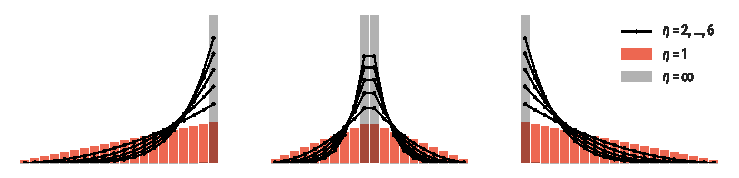
\includegraphics[trim=0.26cm 0 0 \figtopmargin]{FIG03-illustration-eta}
	\caption{Exponentiating a distribution moves the probability mass towards the mode. Illustrated for three different distributions.
		\figdetails{\figid{fig03}}
		\label{fig:FIG03}}
\end{SCfigure}
%- - - - - - - -




%——————————————————————————————————————————————————————————
\paragraph{The emergence of compositionality, ii}

It might be helpful to go through a concrete example.
\textcite{Griffiths2005} introduced a ‘binary’ language, which figured in several later studies \parencite{Griffiths2007,Burkett2010,Kirby2015}.
It is a special case of the shape-color example introduced earlier, with two colours and two shapes (so $F=V=2$).
The language was introduced to study the emergence of compositionality.
If we simplify the encoding, it is easier to see what the compositional languages are.
Write 0 for a triangle, 1 for a square, 0 for black and 1 for orange, such that  $(\square, \orcl)$ for instance becomes $10$ and $(\triangle, \blcl)$ becomes $01$.
Using alphabet $\{a, b\}$ there are 4 compositional languages given by the  feature-subsignal mappings
%-
\begin{align*}
	&(1)\qquad    0 \mapsto a, \quad 1\mapsto a \\
	&(2)\qquad    0 \mapsto a, \quad 1\mapsto b \\
	&(3)\qquad    0 \mapsto b, \quad 1\mapsto a \\
	&(4)\qquad    0 \mapsto b, \quad 1\mapsto b
\end{align*}
%-
In this scenario there are 4 meanings ($\bltr,\ortr,\blsq,\orsq$) and $4^4 = 256$ ways to map four meanings to four signals $\{aa, ab, ba, bb\}$. 
This gives 256 languages of which 4 compositional and 252 holistic.
%%





Not all languages are equally likely. 
A hierarchical prior that puts a fraction $\alpha$ of the probability mass on the compositional languages:
%-
\begin{equation}
    p(\lang) = \begin{cases}
        \frac{\alpha}{4}  		&\text{if $\lang$ is compositional}\\
        \frac{1-\alpha}{256} 	&\text{otherwise}
    \end{cases}
\end{equation}
%-
Once an language $\lang$ has been fixed, the agent is presented with new meaning $m$ for which it then produces a signal $s$ by sampling from the distribution
%-
\begin{equation}
    p(s \mid m, z) = \begin{cases}
        1-\epsilon 				&\text{if $m \mapsto s$ in language $\lang$}\\
        \nicefrac{\epsilon}{3} 	&\text{otherwise}
    \end{cases}
\end{equation}
%-
This means the agent will pick the signal $s$ corresponding to $m$ under language $\lang$ most of the time, but has a small probability $\epsilon$ of making an error and uniformly picking one of the other signals. 
Together with a completely independent distribution $p(m)$, typically a uniform one, this specifies the production algorithm
%-
\begin{align}
	p_{\PA}(x \mid \lang) 
		&= p(s \mid m, \lang) \cdot p(m), 
	\qquad \obs = (m,s)
\end{align}
%-
If $\vobs = ((m_1, s_1), \dots (m_b, s_b))$ is the list of the utterances produced by the previous agent, then the posterior distribution is
%-
\begin{align}
	p(\lang \mid \vobs) 
		&\propto p(\lang) 
			\cdot \prod_{i=1}^b p_{\PA}(\obs_i \mid \lang),
\end{align}
%-
and, as usual, the language algorithm takes the form $p_{\LA}(\lang \mid \vobs) \propto p(\lang \mid \vobs)^\eta$.
%%




%- - - - - - - -
\begin{SCfigure}
	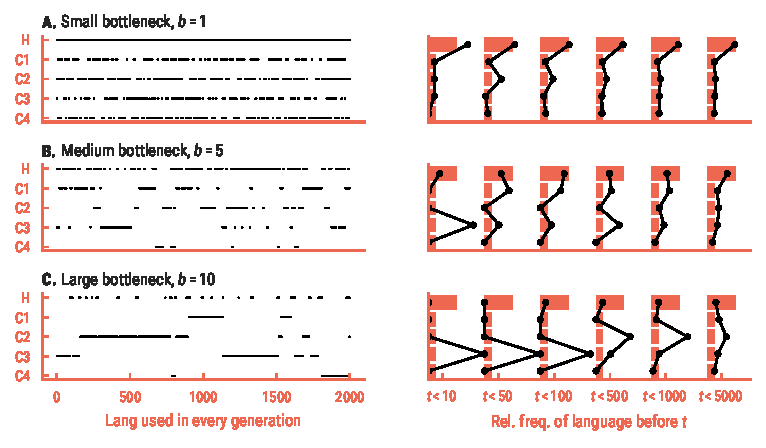
\includegraphics[trim=.7cm 0 0 \figtopmargin]{GK01-bottlenecks}
	
	\caption{
	Emergence of compositionality in the Bayesian iterated learning model of \textcite{Griffiths2007a}.
	On the left, the language used in every generation with H one of 252 holistic languages and C1--4 the compositional languages. 
	On the right the relative frequency of every language up to a certain time $t$.
	These relative frequencies converge to the prior (orange).
	Larger bottlenecks (subfigures A--C) slow down convergence.
	%----------
	\figdetails{\figid{gk01} 
	WebPPL simulation with $\alpha=0.5$, $\epsilon=0.001$ and samplers ($\eta=1$).}
	\label{fig:GK01-bottlenecks}}
\end{SCfigure}
%- - - - - - - -


Figure \ref{fig:GK01-bottlenecks} illustrates the resulting simulation in a population of samplers ($\eta=1$).
It shows which language was used in every generation (left): one of the 252 holistic languages (H) or a compositional language (C1--4).
The compositional languages seem to be used much more frequently, which is confirmed by the plots on the right.
There we see the relative frequency of every language up to several points $t$ in the simulation.
These plots indicate that the relative frequencies converge to the prior, shown in orange.
Since the compositional languages have a higher prior probability than each of the holistic languages, they are more frequent.
The convergence rate towards the prior is much faster when the bottleneck is small ($b=1$, subfigure A) than when it is large ($b=10$, subfigure C).
It is clear why this happens: the more data is transmitted, the greater the probability that the child can reconstruct the language.
The result is that languages will be stable throughout multiple generations, as seen from the lines in figure \ref{fig:GK01-bottlenecks}\textsc{c}.
Nevertheless, even with a large bottleneck the relative frequencies seem to converge to the prior, be it very slowly.
We will discuss all these findings in more detail later. 
First, what discuss the observed ‘convergence to the prior’.
%%




%——————————————————————————————————————————————————————————
%——————————————————————————————————————————————————————————
\section{Convergence to the prior}
%——————————————————————————————————————————————————————————
%——————————————————————————————————————————————————————————



Let me briefly summarise what we have seen so far.
Bayesian agents observe utterances $\obs_{t-1}$ produced by the previous agent, and then use Bayes’ rule to infer a language.
This language is $\lang$ is drawn from $p_\eta(\lang_t \mid \obs_{t-1}) = p(\lang_t \mid =\obs)^\eta$, where $\eta$ interpolates between a sampling- and \textsc{map}-strategy for $\eta=1$ and $\eta = \infty$ respectively.
All this results in a chain  of the form
%-
\begin{equation}
	\label{eq:iterated-learning-chain}
	%-----
	\obs_0 
		\longrightarrow \lang_1 
		\longrightarrow \obs_1 
		\longrightarrow \lang_2 
		\longrightarrow \obs_2 
		\cdots.
\end{equation}
%-
\textcite{Griffiths2005} noted that several Markov chains can be discerned in \eqref{eq:iterated-learning-chain}, of which the long-term behaviour is well-studied: 
They often converge to a so called stationary distribution.
This characterised the long-term behaviour of the iterated learning model.
%%




Appendix \ref{app:markov-chains} introduces the relevant convergence results for Markov Chains; I only summarise them here.
Consider a system with a set of possible states $S$.
If the variables $x_0, x_1, x_2, \dots$ indicate the state at every time step, they form a Markov chain if the probability of moving to another state only depends on the last state: $p(x_t \mid x_0, \dots, x_{t-1}) = p(x_t \mid x_{t-1})$.
If the number of states is finite, these \emph{transition probabilities} can be collected in the transition matrix $\vect T$.
Suppose the initial distribution over states is given by vector $\vecpi$, then the next distribution is $p(x_1 = i) = (\vect T \vecpi)_i$ and after $t$ steps, $p(x_t = i) = (\vect T^t \vecpi)_i$. 
These probabilities can converge to the so called \emph{stationary distribution} $\vecpi^\star$ which must be an eigenvector of $\vect T$ since $\vect T \vecpi^\star = \vecpi^\star$.
If the Markov chain is \emph{ergodic} it is guaranteed to have a unique stationary distribution to which it converges: $p(x_t = i) \to \vecpi^\star_i$ as $t\to\infty$.
Ergodicity, briefly, ensures that the chain keeps revisiting the entire state space and has a positive probability of reaching any other state from any given state in a finite number of steps.
How often it visits every state is given by the stationary distribution, in the sense that the relative frequencies of visited states converges to the stationary distribution.




%- - - - - - -
\begin{SCfigure}
	%\documentclass{../src/bcthesispart}
%\begin{document}
\begin{tikzpicture}[xscale=2.2,yscale=1.2]\sffamily\footnotesize
	\tikzset{lang/.style={draw, circle, fill=main!20}}
	\tikzset{obs/.style={draw, circle, fill=main}}
	\tikzset{obslang/.style={draw, circle, fill=main!60}}
	\tikzset{produce/.style={thick,draw,->}}
	\tikzset{limit/.style={draw,->,dashed}}
	\tikzset{formula/.style={midway,above}}
	
	% Chain
	\begin{scope}
		\path 	(0,0) node[obs]  (x0) {$\obs_0$}
				(1,0) node[lang] (z1) {$\lang_1$}
				(2,0) node[obs]  (x1) {$\obs_1$}
				(3,0) node[lang] (z2) {$\lang_2$}
				(4,0) node[obs]  (x2) {$\obs_2$};			
		\draw[produce]  (x0) -- node[formula] {$p_{\LA}(\lang \mid \obs)$}  (z1);
		\draw[produce] (z1) -- node[formula] {$p_{\PA}(\obs \mid \lang)$} (x1);
		\draw[produce]  (x1) -- node[formula] {$p_{\LA}(\lang \mid \obs)$}  (z2);
		\draw[produce] (z2) -- node[formula] {$p_{\PA}(\obs \mid \lang)$} (x2);
	\end{scope}
	
	% Chain on languages
	\begin{scope}[yshift=-1cm]
		\path 	(1,0) node[lang] (z1) {$\lang_1$}
				(3,0) node[lang] (z2) {$\lang_2$}
				(5,0) node (limit) {$p(\lang)$};
		\draw[produce] (z1) -- node[formula] {$\sum_\obs p_{\LA}(\lang \mid \obs)\cdot p_{\PA}(\obs \mid \lang)$} (z2);
		\draw[limit] (z2) -- (limit);
	\end{scope}

	% Chain on productions
	\begin{scope}[yshift=-2cm]
		\path 	(0,0) node[obs]  (x0) {$\obs_0$}
				(2,0) node[obs]  (x1) {$\obs_1$}
				(4,0) node[obs]  (x2) {$\obs_2$}
				(5,0) node (limit) {$p(\obs)$};			
		\draw[produce]  (x0) -- node[formula] 
			{$\sum_\lang p_{\PA}(\obs \mid \lang) \cdot p_{\LA}(\lang \mid \obs)$}  (x1);
		\draw[produce]  (x1) -- node[formula] 
			{$\sum_\lang p_{\PA}(\obs \mid \lang) \cdot p_{\LA}(\lang \mid \obs)$}  (x2);
		\draw[limit] (x2) -- (limit);
	\end{scope}
	
	% Chain on pairs
	\begin{scope}[yshift=-3cm]
		\path 	(1,0) node[obslang] (zx1) {$\lang_1, \obs_1$}
				(3,0) node[obslang] (zx2) {$\lang_2, \obs_2$}
				(5,0) node (limit) {$p(\lang,\obs)$};
		\draw[produce] (zx1) -- node[formula] {$p_{\LA}(\lang \mid \obs)\cdot p_{\PA}(\obs \mid \lang)$} (zx2);
		\draw[limit] (zx2) -- (limit);
	\end{scope}
\end{tikzpicture}
%\end{document}
	
	\caption{Different Markov chains hidden in the Bayesian iterated learning model, and to which stationary distribution they converge (right).
	%----------
	\figdetails{Figure adapted from \textcite{Griffiths2007a}.}
	\label{fig:gk-markov-chains}}
\end{SCfigure}
%- - - - - - -




%——————————————————————————————————————————————————————————
\paragraph{Proof of the convergence to the prior}

\textcite{Griffiths2005} noted that by marginalising out the productions $\obs_t$ in \eqref{eq:iterated-learning-chain} one obtains the following Markov chain (see also figure \ref{fig:gk-markov-chains}):
%-
\begin{align}
	p(\lang_t \mid \lang_{t-1}) 
		= \sum_{\obs_{t-1}} 
			p_{\LA}(\lang_t \mid \obs_{t-1}) 
			\cdot p_{\PA}(\obs_{t-1} \mid \lang_{t-1}).
	%-----
	\label{eq:mc-interpretations}
\end{align}
%-
We hitherto assumed that the transition probabilities remain constant over time, that is, we looked at time-homogeneous chains. 
The Markov chain in \eqref{eq:mc-interpretations} is only homogeneous if all agents use the same production and language algorithms. 
In particular, they should all use the same prior.
We will later discuss the validity of this assumption. 
If these assumptions hold and the chain is moreover ergodic, \emph{then} the long-term behaviour of iterated learning is known: convergence to the stationary distribution, independent of the initial distribution.





The stationary distribution $\vecpi^\star$ of this distribution happens to be the prior $q(\lang) := p(\lang)$.
To show this, one has to see that
%-
\begin{equation}
	\label{eq:to-prove-convergence}
	%-----
	q( \lang_{t+1}) 
		= \sum_{\lang_t} 
			p(\lang_{t+1} \mid \lang_t) 
			\cdot q(\lang_t)
\end{equation}
%-
I have written $q$ for the prior to highlight that we do not know whether $q(\lang_{t+1})$ is a marginal distribution of $p(\lang_{t+1}, \lang_t)$.
In that case, the equality would hold trivially.
Otherwise, the following derivation shows that \eqref{eq:to-prove-convergence} holds:
%-
\begin{align}
	\label{eq:proof-conv-to-the-prior}
	%-----
	\sum_{\lang_t} 
		q(\lang_t) 
		\cdot p(\lang_{t+1} \mid \lang_t)
		%
		&= \sum_{\lang_t} 
				q(\lang_t) \cdot \sum_{\obs_t} 
					p_{\LA}(\lang_{t+1} \mid \obs_t)  
					\cdot p_{\PA}(\obs_t \mid \lang_t)
		\\
		&= \sum_{\obs_t} 
				p_{\LA}(\lang_{t+1} \mid \obs_t) 
				\cdot \sum_{\lang_t} 
		   			q(\lang_t) 
		   			\cdot p_{\PA}(\obs_t \mid \lang_t)
		\\\nonumber
		&= \sum_{\obs_t} 
			p_{\LA}(\lang_{t+1} \mid \obs_t) 
			\cdot p_{\PA}(\obs_t)
		\\\nonumber
		&\overset{(\star)}{=} 
			\sum_{\obs_t} 
				\frac{p_{\PA}(\obs_t \mid \lang_{t+1}) \cdot q(\lang_{t+1})}%
				{p_{\PA}(\obs_t)} \cdot p_{\PA}(\obs_t)
		\\\nonumber
		&= q(\lang_{t+1}) 
			\sum_{\obs_t} 
				p_{\PA}(\obs_t \mid \lang_{t+1})
		\\\nonumber
		&= q(\lang_{t+1}) 
\end{align}
where $(\star)$ holds by definition of $p_{\LA}(\lang_{t+1} \mid \obs_t)$ and because we use samplers ($\eta=1$).
For maximisers, the proof breaks down at this point.
%%





Similar results hold for the other Markov chains hidden in the iterated learning model (see figure \ref{fig:gk-markov-chains}).
When averaging over interpretations rather than productions, one obtains a Markov chain on the productions:
%-
\begin{align}
	p(\obs_{t+1} \mid \obs_t) 
		= \sum_{\lang_{t+1}} p(\obs_{t+1} \mid \lang_{t+1}) 
			\cdot p(\lang_{t+1}\mid \obs_t).
\end{align}
%-
A proof analogous to \eqref{eq:proof-conv-to-the-prior} shows that this chain converges to the \emph{prior predictive distribution} $p(\obs)  =  \sum_{\lang} p_{\PA}(\obs \mid \lang) \cdot p(\lang)$
Finally, one could consider a Markov chain over the state space of language-utterance pairs $(\lang, \obs) \in \langspace\times \obsspace$ with transition probabilities
%-
\begin{align}
	\label{eq:chain-joint}
	%-----
	p(\lang_{t+1}, \obs_{t+1} \mid \lang_t, \obs_t) 
		= p(\lang_{t+1} \mid \obs_t) 
			\cdot p(\obs_t \mid \lang_t).
\end{align}
%-
This chain has the joint $p(\lang, \obs) = p_{\PA}(\obs \mid \lang) \cdot p(\lang)$ as its stationary distribution.
Interestingly, this shows that Bayesian iterated learning implements a \emph{Gibbs sampler}.




Gibbs samplers are often used in Bayesian statistics, whenever it is not possible to work with complicated distributions analytically.
\emph{Monte Carlo methods} are work-arounds that collect many samples from the distribution, and approximate the distribution using those samples.
To obtain samples, one constructs a Markov chain whose stationary distribution is the distribution of interest.
Over time, the visited states will be (correlated) samples from the target distribution.
This is the basic idea behind many \emph{Markov Chain Monte Carlo} (\textsc{mcmc}) methods and Gibbs sampling is one of those.
It can be used to approximate a joint distribution $p(\lang,\obs)$ if it is easy to sample from the conditional distributions $p(\lang\mid\obs)$ and $p(\obs\mid\lang)$.
In every iteration, it fixes one of the variables, say $\lang_t$ and samples a new $\obs_{t+1}$ from $p(\obs_{t+1}\mid\lang_t)$. 
Then it fixes $\obs_t$ and samples $\lang_{t+1}$ from $p(\lang_{t+1}\mid \obs_{t+1})$, and so on.
This results in a new sample $(\lang_{t+1}, \obs_{t+1})$ from the joint after every ‘sweep’ through the variables.
Indeed, this procedure exactly mirrors Bayesian iterated learning with sampling agents, and it follows that the chain in \eqref{eq:chain-joint} converges to $p(\lang, \obs)$ (see \cite{Griffiths2007a} for a longer discussion).
%%




%——————————————————————————————————————————————————————————
\paragraph{Convergence to the maximum of the prior?}

What kind of behaviour should one expect in populations of maximisers?
This turns out to be a much harder question.
There are, to the best of my knowledge, two analytical results — we will return to empirical evaluations in chapter \ref{ch:bayesian-naming-games} — both suggesting that in populations of maximisers the behaviour is largely determined by the prior, but in a less direct way.
First of all, \textcite{Kirby2007} analyses the stationary distribution for maximisers ($\eta>1$) using a constrained set of languages that spread the probability mass uniformly over a (sub)set of utterances.\footnote{%
	%>>>
	This constraint on languages has a purely mathematical motivation: it is precisely what is needed to factorise the normalising constant in the posterior.
	%<<<
	}
In other words, $p(\obs \mid \lang)$ is either 0 or equal to a $f(\obs)$, where the latter does not depend on $\lang$.
In that case, the stationary distribution is proportional to $p(z)^\eta$.
This implies that cultural evolution results in an exaggerated version of the prior (cf.~figure \ref{fig:FIG03}).




A similar conclusion follows from the second result, due to \textcite{Griffiths2007a}.
They note that maximisers (now $\eta=\infty$) implement a version \emph{Expectation-Maximisation} (\textsc{em}).
This is an iterative algorithm used in models with hidden variables to estimate parameters that are increasingly close to the maximum likelihood estimates, or, in our case, \textsc{map} estimates.
The trick is to use the current parameters to estimate the \emph{expected} likelihood of the observed and hidden variables, and then update the parameters so that they \emph{maximize} that likelihood.
When computing the expectation analytically is intractible, it can be approximated by drawing several samples.
The case using a single sample is called \emph{stochastic \textsc{em}}.
Now, suppose, in \textsc{em} jargon, there are no observed variables, $\obs_t$ is the latent variable and $\lang_t$ the parameter, then stochastic \textsc{em} in this model amounts to Bayesian iterated learning in a population of maximisers (see \textcite{Griffiths2007a} for details).
This characterisation is not as clear-cut as with samplers, but suggests that the stationary distribution over languages will roughly be centred on the maxima of the prior \parencite{Griffiths2007a}.
%%






%——————————————————————————————————————————————————————————
%——————————————————————————————————————————————————————————
\section{Convergent controversy}
%——————————————————————————————————————————————————————————
%——————————————————————————————————————————————————————————


The \emph{convergence to the prior} was the first general result about the long-term behaviour of the iterated learning model.
For populations of samplers, the result was crystal clear: starting from any initial distribution, the probability that an agent down the chain would be using language $\lang$ is given by the prior probability $p(\lang)$.
And this is precisely what we observed in figure \ref{fig:GK01-bottlenecks}, which shows the the emergence of compositionality — or rather, the emergence of the prior.
The model is an ergodic Markov chain, and over time the probability that a certain language will be used therefore converges to its probability under the stationary distribution, which is the prior.
Compositional languages have high probability under that prior, and consequently emerge.
Maximisers are much harder to analyse.
The probability that a language is used by maximisers seems to be largely determined by the maxima of the prior.
Now, what are the implications of all this for cultural language evolution?

%The Bayesian model elicited a response from many researchers in the field, questioning the assumptions and interpretations offered by Griffiths and Kalish.
%%




%——————————————————————————————————————————————————————————
\paragraph{Bottlenecks and weak biases}

Iterated learning was inspired by the idea that language is a compromise between “the biases of learners, and other constraints acting on language during their transmission” \parencite{Smith2009}, originally in the form of a transmission bottleneck.
But in the Bayesian models, the bottleneck hardly plays any role.
\textcite{Griffiths2007a} conclude that “the emergence of languages with particular properties does not require a bottleneck” (p.~466).
Larger bottlenecks do slow down convergence since they imply more faithful transmission and this increases language stability.
The Markov chain’s walk through the state space consequently slows down, which, somewhat paradoxically, also slows down convergence. 
But in the long run bottlenecks play no role — at least for samplers.
This seems to undermine the idea that compressible languages emerge \emph{because of} cultural transmission.
Should we conclude, then, that languages are not shaped by cultural evolution, but primarily by innate constraints?
\textcite{Griffiths2007a} conclude that their results “do not indicate which of these explanations is more plausible” (p.~475).
There’s something for everyone: if the prior captures innate biases, “iterated learning acts as an engine by which these constraints result in universals” (p.~475), but if you prefer the transmission process to actually change the priors, then you “can take heart from our results for learners who use \textsc{map} estimation”.
%%





\textcite{Kirby2007} follow the latter advise. 
Their paper discusses an iterated learning model with maximisers that have a prior bias towards regular languages.
Bottleneck effects can occur in populations of maximisers \parencite{Griffiths2007a} and the authors accordingly conclude that as the bottleneck tightens in their model, “regularity is increasingly favoured”. 
But there is something peculiar about this conclusion: 
It seems to hold only because their prior favoured regularity.
Had their prior favoured irregularity, irregularity would have been increasingly favoured under a tighter bottleneck.\footnote{%
	%>>>
	I found their \textsc{pnas} paper is a bit sketchy on the details of their simulations, but these conclusions follow directly from \textcite{Griffiths2007a} and as far as I can see apply equally to \textcite{Kirby2007}.
	%<<<
	}
In the Bayesian model, transmission at most amplifies pre-existing biases, which of course can be seen as an effect of cultural transmission. 
Another conclusion of \textcite{Kirby2007} is therefore that processes of cultural evolution can “completely obscure” the \emph{strength} of the bias.
A small tendency to favour languages with higher prior probability (i.e.\ $\eta>1$) amplifies weak biases and results in strong universals. 
The strength of the bias has no role, only the ordering of the languages.
All in all, it suggests a rather toothless process of cultural evolution.
Several researchers therefore started tweaking the assumptions of the model to find out how robust the results are.
%%




%——————————————————————————————————————————————————————————
\paragraph{population structure and heterogenous populations}

The population structure was one of the first things addressed.
It should be noted that \parencite{Griffiths2007a} generalised their findings to somewhat different scenario, with finite generations evolving in (discrete or) continuous time \parencite[cf.][]{Nowak2001}.
In that case the \emph{proportion} $p_t(\lang)$ of the population speaking language $\lang$ at time $t$ converges to the prior $p(\lang)$, as can easily be seen.
If $\vect p_t = (p_t(\lang): \lang\in \langspace)$ and $\vect T$ the transition matrix, these proportions change as
\begin{equation}
	\vect p_{t+1} = \vect T \vect p_t,
\end{equation}
which describes a linear dynamical system with a unique stable equilibrium.
The same derivations as \eqref{eq:proof-conv-to-the-prior} show the prior is that equilibrium. 
However, \textcite{Niyogi2009} argue that this is an unrealistic model of language evolution as it precludes the possibility of bifurcations.
Moreover, language stability cannot be maintained: even if only 0.01\% of the population uses a different language, it will spread to a larger share of the population (the prior admitting).
As a remedy \textcite{Niyogi2009} propose an alternative model where agents learn from a mixture of the languages used in the previous generation, not just one.
This leads to markedly different nonlinear behaviour with bifurcations and possibility multiple equilibria, which they argue accurately describes historical developments (namely, that English is no longer a ‘verb-second’ language).
%%
%Now bifurcations \emph{do} occur and they argue this accurately describes an historical example (that English is no longer a ‘verb-second’ language).




That the behaviour changes in different populations structures was confirmed in several other studies.
\textcite{Smith2009} similarly considered infinite generations of agents learning from multiple parents.
He reports that this precludes convergence to the prior and introduces a dependency on the initial distribution of languages in the population.
\textcite{Ferdinand2009} draw the same conclusion, but also drop the assumption that all agents share the same innate biases, i.e. that the population is \emph{homogeneous}.
In heterogeneous population the convergence to the prior breaks down.
\textcite{Dediu2009} finds that the strong differences between samplers and maximisers disappears in populations with a different structure or heterogeneity.
%%




The agents in studies such as \textcite{Ferdinand2009} are not Bayesian agents in the strict sense that agents assume to be learning from a single language, while in fact the data comes from several sources.
\textcite{Burkett2010} address this issue in a hierarchical model where agents take into account that they are possibly learning from multiple languages.
Accordingly, the convergence to the prior reappears.
Very recently, \textcite{Whalen2017} extended this to populations with arbitrary network structures, although it should be stressed that agents still learned from a single teacher.
Nevertheless, the emerging consensus appears to be that in slightly more complicated population structures (with possibly imperfect Bayesian reasoners) the convergence to the prior can break down and nontrivial cultural effects appear.
%%






%——————————————————————————————————————————————————————————
\paragraph{Lineages and cumulative cultural evolution}

It is somewhat surprising that the population structure received most criticism, since that aspect of the Bayesian model is perfectly in line with the original iterated learning model.
Some other parts, I would argue, are not.
First of all, the type of convergence — in language or in probability of using a language — is markedly different.
In early iterated learning studies, the population converged to a stable language which could be transmitted faithfully along many generations.
In the Bayesian models, nothing of this sort happens.
In the simulation of the emergence of compositionality (figure \ref{fig:GK01-bottlenecks}) one clearly sees that successive generations can acquire radically different languages: picture English-speaking parents, themselves born to Basque parents, whose children miraculously learned Hungarian.
%%




Transmission in the Bayesian model generally not faithful — indeed, this is  necessary for ‘convergence’ to occur at all.
That seems particularly problematic for a model of cultural evolution.
Even if transmission shapes languages, it has to be somewhat faithful if one expects any kind of cultural \emph{evolution}.
\textcite{Tomasello1999} points out that faithful transmission is important because it enables a so called \emph{cultural ratchet}, where cultural innovations are passed on and improved upon by later generations.
Cultural evolution, as a result, is \emph{cumulative} and products of cultural evolution consequently reflect their full historical development.
If it is not already uneasy that the defining property of a Markov chain is being memoryless, ergodicity certainly conflicts with the idea of cumulative cultural evolution.
In an ergodic Markov chain, every ‘lineage’ is guaranteed to revisit all possible languages infinitely often.
That amounts to an infinite reinvention of the wheel — pretty much the exact opposite of cumulative cultural evolution.
%%




%——————————————————————————————————————————————————————————
%——————————————————————————————————————————————————————————
\section{Conclusions}
%——————————————————————————————————————————————————————————
%——————————————————————————————————————————————————————————


The first iterated learning models suggested that languages primarily pick up systematicity during cultural transmission.
Simulations showed how compositional structure accumulated in initially unstructured languages when a bottleneck pressured the languages to become more compressible.
However, the learning algorithms that generalise a few observations to a full language implement all kinds of implicit biases, and possibly provide an implicit pressure towards compositional structures.
To make general claims about the interaction of cultural processes and innate biases, the two need to be separated clearly.
Bayesian iterated learning models did precisely that, but were also shown to \emph{converge to the prior}.
That meant that the probability that a certain language would be used, is after a while completely determined by the biases of the learners, independent of the initial conditions.
In populations of maximisers, the relation is less transparent and the shape of the prior (its maxima in particular) largely appears to determine the outcome of cultural evolution.
%%




The Bayesian iterated learning model moved the explanatory load from the cultural process to the prior biases of the learners.
However, the strong conclusions were in several studies shown to break down in more complicated populations.
The Bayesian model moreover results in an arguably unrealistic model of cultural evolution, with no language stability, nor any cumulative effects.
Despite these shortcomings, the field made significant progress due to the work of Griffiths and Kalish.
Explicitly encoding the biases of the learners made studies of the interactions between the ‘nature’ and ‘nurture’ of language much more principled, and moreover resulted in cognitively better motivated agents.
The focus on analytic results regarding the long-term behaviour brought further transparency to the somewhat opaque conclusions suggested by simulations alone — irrespective of whether the results are ultimately convincing.



\bigbreak\noindent
In sum, combining the criticism and benefits, I would draw up the following list of desiderata for a model that aims to show that cultural processes can shape the evolution of language (in arbitrary order):
%...
\begin{enumerate}[label=(\textsc{d}\arabic*)]
	\item \textbf{Explicate biases.}
	\label{desideratum:biases}
	The biases of the agents should be explicitly specified in the model.
		
	\item \textbf{Strategies.}
	\label{desideratum:strategies}
	The model should explore a wide range of strategies, such as sampling or \textsc{map} strategies.
	
	\item\textbf{Analysable.}
	\label{desideratum:analysable}
	The model should be amenable to analytical scrutiny, and it should ideally be possible to draw general conclusions about long-term behaviour.
	
	\item \textbf{Nontrivial cultural effects.}
	\label{desideratum:cultural-effects}
	The model should exhibit non-trivial cultural effects, which might for example result in lineage-specific evolution: different runs resulting in different outcomes of cultural evolution.
	
	\item \textbf{Robustness to population structure.}
	\label{desideratum:robust}
	The model should exhibit behaviour that is fairly robust to changes in population structure.
	
	\item \textbf{Language stability.}
	\label{desideratum:stable}
	The model should result in a ‘reasonable’ degree of language stability. Reasonable, since languages are never perfectly stable \parencite[see also][]{Kirby2001}.
	
	\item \textbf{Empirically testable.}
	\label{desideratum:empirical}
	The model should give an empirically plausible, mechanistic explanation of cultural evolution, which is further testable against empirical linguistic findings (predating the lab).
\end{enumerate}
%...
The list is no doubt incomplete, but mainly serves as a guide to what I will address in this thesis, most notably in chapter \ref{ch:bayesian-naming-games}.




% Print the bibliography
\showbibliography

\end{document}



%%% TODO WAAR MOET DIT HEEN?!?!

In this context a later paper by Kirby and colleagues should be mentioned.
%Recall that the most compressible language is a degenerate language with a single word.
%Now, in laboratory experiments with humans that closely mirror iterated learning chains, \textcite{Kirby2008} found that languages became better transmissible, but sometimes by degenerating to highly ambiguous languages, using a few words for many different objects.
Over the last decade, experimental studies closely mirroring the iterated learning setup, revealed that a pressure for compressibility alone does not give rise to compositional languages \parencite{Kirby2008}.
We for example already discussed the degenerate, one-word languages which is highly compressible, but not \emph{expressive}.
Recently, \textcite{Kirby2015} therefore concluded that a pressure for \emph{compressibility} has to be counterbalanced by a pressure for \emph{expressivity}, in order for compositional structure to emerge.
The idea that compositional structure balances compressibility and expressivity was later translated to the Bayesian modelling tradition in \textcite{Kirby2015}.
They did so by using a prior that favoured compressible languages, and introduced a parameter that penalises ambiguous languages.
Their model also added a population structure that would, they anticipated, implement a pressure for expressivity, 




%todo (optional) refer to Dunn 2011?
%This can be turned into an empirical argument. The Bayesian iterated learning model with samplers after all “suggests  transparent relationship between the prior bias of the learners and the observed distribution of languages in the world: the typological distribution exactly reflects the biases of learners” \parencite{Smith2009}.

%todo (optional) include “This suggests a transparent relationship between the prior bias of learners and the observed distribution of languages in the world: the typological distribution exactly reflects the biases of learners”. SMITH 2009
